
\documentclass[10pt,conference]{IEEEtran}

\addtolength{\topmargin}{-2mm} \addtolength{\topskip}{-2mm} \addtolength{\textheight}{+5mm}
\addtolength{\textwidth}{+2mm}
\addtolength{\textfloatsep}{-3mm}
\addtolength{\columnsep}{-1mm}
\addtolength{\topsep}{-1mm}
\addtolength{\textfloatsep}{-3mm}



\usepackage{amsmath}

\usepackage[english]{babel}
\usepackage[utf8]{inputenc}
\usepackage{multirow}
\pagestyle{empty}
\usepackage{graphicx}
\usepackage{float}
\usepackage{tabu}
\usepackage{eurosym} \usepackage{color} \usepackage{soulutf8} \usepackage{amsmath} \usepackage[nolist]{acronym}
\usepackage[caption=false,font=footnotesize]{subfig}
\usepackage{sidecap} 
\hyphenation{op-tical net-works semi-conduc-tor}



\newcommand{\LONG}[1]{}
\RequirePackage[normalem]{ulem} \RequirePackage{color}\definecolor{RED}{rgb}{1,0,0}\definecolor{BLUE}{rgb}{0,0,1} \providecommand{\DIFadd}[1]{{\protect\color{blue}\uwave{#1}}} \providecommand{\DIFdel}[1]{{\protect\color{red}\sout{#1}}}                      \providecommand{\DIFaddbegin}{} \providecommand{\DIFaddend}{} \providecommand{\DIFdelbegin}{} \providecommand{\DIFdelend}{} \providecommand{\DIFaddFL}[1]{\DIFadd{#1}} \providecommand{\DIFdelFL}[1]{\DIFdel{#1}} \providecommand{\DIFaddbeginFL}{} \providecommand{\DIFaddendFL}{} \providecommand{\DIFdelbeginFL}{} \providecommand{\DIFdelendFL}{} 
\begin{document}







\title{Shuttle: Intrusion Recovery for PaaS}
\author{
	\IEEEauthorblockN{Dário Nascimento, Miguel Correia}\\
	\IEEEauthorblockA{INESC-ID, Instituto Superior Técnico, Universidade de Lisboa\\
		\{dario.nascimento,miguel.p.correia\}@tecnico.ulisboa.pt}
	}

\maketitle

\thispagestyle{plain}
\pagestyle{plain}

\ifCLASSOPTIONpeerreview
\begin{center} \bfseries Regular Paper \end{center}
\fi
\IEEEpeerreviewmaketitle



\begin{acronym}[IHE]
		\acro{ACID}{\emph{Atomicity, Consistency, Isolation and Durability}}
	\acro{API}{\emph{Application Programming Interface}}
	\acro{AWS}{\emph{Amazon Web Services}}
	\acro{BDB}{\emph{Berkeley DB}}	
	\acro{CAP}{\emph{Consistency, Availability, Partition Tolerance}}
	\acro{CPU}{\emph{Central Processing Unit}}
	\acro{CRUD}{\emph{create, read, update and delete}}
	\acro{CSP}{\emph{Cloud service providers}}
	\acro{DBMS}{\emph{Database Management System}}
	\acro{DFS}{\emph{Deep First Search}}	
	\acro{DHT}{\emph{Distributed Hashtable}}	
	\acro{DOM}{\emph{Document Object Model}}
	\acro{EBS}{\emph{Elastic Block Store}}
	\acro{EC2}{\emph{Elastic Compute Cloud}}
	\acro{ECU}{\emph{EC2 Compute Unit}}
	\acro{ELB}{\emph{Elastic Load Balancer}}	
	\acro{HTTPS}{\emph{Hypertext Transfer Protocol Secure}}
	\acro{HTTP}{\emph{Hypertext Transfer Protocol}}
	\acro{IaaS}{\emph{Infrastructure as a Service}}
	\acro{IDL}{\emph{Interface Description Language}}
	\acro{IDS}{\emph{Intrusion detection system}}
	\acro{IMAP}{\emph{Internet Message Access Protocol}}
	\acro{IOPS}{\emph{Input/Output Operations Per Second}}	
	\acro{IP}{\emph{Internet Protocol}}
	\acro{JAX-WS}{\emph{Java API for XML Web Services }}
	\acro{JIT}{\emph{Just-in-time}}
	\acro{JVM}{\emph{Java Virtual Machine}}
	\acro{MVC}{\emph{Model View Controller}}
	\acro{NIO}{\emph{Non Blocking IO}}	
	\acro{NIST}{\emph{National Institute of Standards and Technology}}
	\acro{NoSQL}{\emph{Not only SQL}}
	\acro{OWASP}{\emph{Open Web Application Security Project}}	
	\acro{PaaS}{\emph{Platform as a Service}}
	\acro{protobuf}{\emph{Google Protocol Buffers}}	
	\acro{QA}[Q\&A]{\emph{Questions and Answers}}
	\acro{RDBMS}{\emph{Relational Database Management System}}
	\acro{REST}{\emph{Representational State Transfer}}
	\acro{RID}{\emph{Request ID}}	
	\acro{RMI}{\emph{Remote Method Invocation}}	
	\acro{RPC}{\emph{Remote Procedure Call}}	
	\acro{S3}{\emph{Simple Storage Service}}
	\acro{SaaS}{\emph{Software as a Service}}
	\acro{SID}{\emph{Snapshot ID}}	
	\acro{SOAP}{\emph{Simple Object Access Protocol}}	
	\acro{SQL}{\emph{Structured Query Language}}
	\acro{SRD}{\emph{Shuttle Request Data}}
	\acro{SSD}{\emph{Solid State Disk}}
	\acro{SSH}{\emph{Secure Shell}}
	\acro{SSL}{\emph{Secure Socket Layer}}
	\acro{TCP}{\emph{Transmission Control Protocol}}
	\acro{TID}{\emph{Thread Id}}
	\acro{VM}{\emph{Virtual Machine}}
	\acro{VPC}{\emph{Virtual Private Cloud}}	
	\acro{YCSB}{\emph{Yahoo! Cloud Serving Benchmark}}
\end{acronym}


\begin{abstract}
The number of applications being deployed using the Platform as a Service (PaaS) cloud computing model is increasing. Despite  the security controls implemented by cloud service providers, we expect intrusions to strike such applications. We present Shuttle, a novel intrusion recovery service. Shuttle recovers from intrusions in applications deployed in PaaS platforms.
Our approach allows undoing changes to the state of PaaS applications due to intrusions, without loosing the effect of legitimate operations performed after the intrusions take place. We combine a record-and-replay approach with the elasticity provided by cloud offerings to recover applications deployed on various instances and backed by distributed databases. The service loads a database snapshot taken before the intrusion and replays subsequent requests, as much in parallel as possible, while continuing to execute incoming requests. 
We present an experimental evaluation of Shuttle on Amazon Web Services. We show Shuttle can replay 1 million requests in 10 minutes and that it can duplicate the number of requests replayed per second by increasing the number of application servers from 1 to 3. 




\end{abstract}


\section{Introduction}
\label{sec:introduction}

\acf{PaaS} is a cloud computing model that supports automated configuration and deployment of applications \cite{Vaquero2008,Vaquero2011}\LONG{Armbrust,Mell}. \ac{PaaS} offerings, such as Google App Engine, Windows Azure, and Force.com, provide an environment \DIFdelbegin \DIFdel{\LONG{model aims to provide an environment} }\DIFdelend in which clients (\textit{tenants}) build and run their application on a managed cloud infrastructure through a set of services. These services are paid-per-usage and \DIFdelbegin \DIFdel{turn the application easy to }\DIFdelend \DIFaddbegin \DIFadd{enable tenants to develop, }\DIFaddend deploy and scale \DIFaddbegin \DIFadd{their applications in production fast}\DIFaddend .

The number of applications running in cloud computing platforms, including those based on the \ac{PaaS} model, is increasing rapidly. Many of these applications are critical for their companies, so the risk of intrusion is high. The recent case of the cloud-based Code Spaces service is conspicuous: hackers deleted most of its data and backups, leading to the termination of the service \cite{McAllister:14}.


Cloud service providers (CSPs) implement several security controls. Most of these controls aim to prevent intrusions: access control, firewalls, intrusion detection and prevention systems, network access control, vulnerability scanning, etc. Despite the importance of these mechanisms, applications often contain design or configuration vulnerabilities that let intrusions happen \cite{Williams2013}\LONG{Hubbard2010}. Complexity and budget/time constraints\LONG{Charette2005}, weak passwords or bad security policies are \DIFdelbegin \DIFdel{known causes of these problems}\DIFdelend \DIFaddbegin \DIFadd{also known causes}\DIFaddend . The recent case of the bash bug (or Shellshock) shows that there are other reasons such as legacy software being used in ways that were unpredictable when it was developed \cite{Sidhpurwala:14}.
Much research has been done on mechanisms to tolerate Byzantine faults, including intrusions \cite{Verissimo2003}\LONG{Castro2002,Gupta:03}. However, most of these techniques do not prevent application level attacks or user mistakes. For instance, if attackers steal legitimate user credentials, they are able to modify the state of the applications violating their security policy. \LONG{In summary, there are several paths for intrusions to happen, even if mechanisms to prevent or tolerate them are used.}


We  assume intrusions can happen and their effects need to be removed from the applications' state. This removal is often done manually by system administrators who have to understand the parts of the state compromised directly by the intrusion or contaminated by operations that used compromised state, before cleaning the state. This process is error-prone, often takes long and causes application unavailability \cite{Brown2001}. Intrusion recovery systems aim to automate these steps and mitigate these issues.

Previous intrusion recovery systems targeted operating systems \cite{taser,retro,dare}, databases \cite{itdb,phoenix}, web applications \cite{Akkus2010,warp,aire} and other services \cite{undoForOperators}. All these works considered one computer plus, in a few cases, a backend server. None of them was designed for cloud applications deployed in multiple servers and using distributed databases. Furthermore, most cause downtime, which is undesirable in online services.

We present a novel \emph{intrusion recovery} service for \ac{PaaS} systems. Shuttle aims to make \ac{PaaS} applications operational despite intrusions, helping tenants to recover their applications from software flaws and malicious or accidentally corrupted user requests without requiring application downtime during the process. When an intrusion is detected, tenants can use Shuttle, provided as a service by CSPs, to remove intrusions' effects and recover the integrity of their applications. This paper concerns application availability and state integrity, not confidentiality.

Shuttle assumes a client-server model in which clients communicate with the servers in the cloud using HTTP / HTTPS. For each application deployed in the \ac{PaaS} system, Shuttle records the requests issued by clients and creates periodic snapshots of the application database. 
After detection of the intrusion, Shuttle loads the snapshot that precedes the beginning of the intrusion and replays only the legitimate requests to recreate an intrusion-free application state. Requests are replayed asynchronously and, whenever possible, concurrently. The recovery process is deterministic because accesses to each data item are performed in the original order of execution.

Dependencies established at database level during the requests' first execution are used to create independent clusters of requests that can be replayed concurrently. We propose a branching mechanism to keep the service executing incoming requests while doing replay.

Unlike previous intrusion recovery systems, Shuttle aims to be provided as a service to applications deployed in \ac{PaaS}. Consequently, it can be well-tested and available without depending on being correctly setup by the application developers. We also leverage the elasticity of \ac{PaaS} infrastructures to reduce the service costs and the recovery period. Specifically, Shuttle is designed to allocate more servers during the recovery period to accommodate the throughput of requests being replayed, and release them at the end, with a proportional impact on service costs. The rapid and continuous decline in computation and storage costs in CSPs makes affordable to store user requests, to use database snapshots and to replay previous requests.

The contributions of this paper are the following: 
(1) a new intrusion recovery approach provided as a service integrated in a \ac{PaaS} system and taking into consideration applications running in various instances backed by distributed databases;
(2) a method to order the replayed user requests considering their accesses to databases;
(3) accomplishing intrusion recovery without service downtime using a branching mechanism;
(4) leveraging the resource elasticity and pay-per-use model in \ac{PaaS} environments to record and launch multiple clients to replay previous non-malicious user requests as concurrently as possible to reduce the recovery time and costs;
(5) a mechanism to do a globally transaction-consistent snapshot of NoSQL databases.

\DIFaddbegin 

\DIFaddend 
\section{Background and Related Work}\label{sec:background}
\DIFdelbegin 
\DIFdel{This section formalizes several approaches to perform intrusion recovery and presents the main related work. 
}\DIFdelend An application execution is modeled as a set of actions $A$ on a set of objects $D$. Actions are described by operations (read, write, others more complex), the value(s) read/written, and a timestamp (which defines the order of the actions). Each object has a state (or value) and a set of operations that can modify it. We define $A_{intrusion}$ as the subset of actions of $A$ whereby the attacker compromises the application during the intrusion \DIFdelbegin \DIFdel{, $A_{after}$ as the subset of actions that began after the intrusion began (including the first action of the intrusion), }\DIFdelend and $A_{legal}$ as the subset of legitimate actions in $A$, i.e., $A_{legal} = A \backslash A_{intrusion}$.

Intrusion recovery services aim to remove the effects of malicious actions setting the application state to a state set only by legitimate actions. 
A \textit{backup} mechanism is a basic recovery service that can set objects to the state they had before an intrusion began. The new state excludes the effects of the attacker's actions, but also the effects of any legitimate actions performed after the backup was done. This second aspect is undesirable, so recent intrusion recovery systems aim to avoid it. This is the case in the \DIFdelbegin \DIFdel{closest works }\DIFdelend \DIFaddbegin \DIFadd{works closest }\DIFaddend to ours: Aire \cite{aire}, Warp \cite{warp}, \DIFaddbegin \DIFadd{Akkus and }\DIFaddend Goel \cite{Akkus2010}, and Undo for Operators (UO) \cite{undoForOperators}. None of these works handles recovery in cloud environments.

An action is considered \textit{tainted} at a certain instant if it \DIFdelbegin \DIFdel{is one of the attacker's malicious actions or if }\DIFdelend \DIFaddbegin \DIFadd{depends on a malicious or tainted action, i.e., }\DIFaddend it reads an object written by a \DIFaddbegin \DIFadd{malicious or }\DIFaddend tainted action (called a \textit{tainted object}). Since actions are contaminated by malicious actions through objects, to remove the state written by tainted actions it is necessary but not sufficient to obtain the state produced by the legitimate actions. \DIFdelbegin 

\DIFdel{Consider a hypothetical application execution. At a certain point in time after an intrusion, the application is stopped and the sequence of actions executed ($A$) is purged of the actions in $A_{intrusion}$.
Then, the state is rewind to the beginning of the application execution and only the actions in $A_{recovered} = A \backslash A_{intrusion} = A_{legal}$ are }\DIFdelend \DIFaddbegin \DIFadd{The tainted actions need to be }\DIFaddend re-executed \DIFdelbegin \DIFdel{. That re-execution is intrusion-free as 
$A \cap A_{intrusion} = \emptyset \implies A_{tainted} = \emptyset$. 
The set of tainted actions of the first execution that are not in $A_{intrusion}$ are re-executed but }\DIFdelend \DIFaddbegin \DIFadd{to }\DIFaddend read different values (not imposed by the attacker) and have a different execution. 
\DIFdelbegin \DIFdel{The replay process restores the application to a correct state $D_{recovered}$, which is not compromised by the intrusion .
}\DIFdelend 


\DIFdelbegin \DIFdel{That generic approach is unfeasible without the use of snapshots.
The sequence of actions performed before the intrusion $A_{before} = A \backslash A_{after}$ can be long and each action takes non-null time to execute, so replaying $A_{before}$ may be unfeasible. Moreover, a log of all the actions executed may be too large. We define the subsets $D_{snapshot}(t)$ and $A_{snapshot}(t) : A_{snapshot}(t) \subset A$ as the subsets of objects and actions executed before the begin of a snapshot operation at instant }\textit{\DIFdel{t}}\DIFdel{. If the intrusion happens after $t$, then $A_{after} \cap A_{snapshot}(t) = \emptyset \implies (A_{intrusion} \cup A_{tainted}) \cap A_{snapshot}(t) = \emptyset$, i.e., the snapshot is not affected by the intrusion. For that reason, the service can replay only $A \backslash A_{snapshot}(t) \backslash A_{intrusion}$ using the object set $D_{snapshot}$ as base. 
}\DIFdelend \DIFaddbegin \DIFadd{There have been different approaches to remove intrusion effects removing the object versions written by malicious actions: Akkus and Goel \mbox{\cite{Akkus2010}
}use transaction compensation (invert transactions' effects) to create snapshots, Warp loads previous data item version and UO loads snapshots. The first approach does not remove the effects of unknown actions, the second requires a considerable storage overhead. We implemented a snapshot mechanism designed for distributed databases. }\DIFaddend 

\DIFaddbegin 

\DIFaddend There are two distinct replay approaches to update \DIFdelbegin \DIFdel{the set of object }\DIFdelend \DIFaddbegin \DIFadd{to a correct state (setting }\DIFaddend $D$ to $D_{recovered}$\DIFdelbegin \DIFdel{, 
}\DIFdelend \DIFaddbegin \DIFadd{): }\DIFaddend selective replay and full replay. 
\DIFdelbegin \DIFdel{A }\textit{\DIFdel{version}} \DIFdel{is a snapshot of a single object value at an instant $t$. Versions can be recorded with the sequence of actions that write the objects before the instant $t$.
}\DIFdelend The \textit{selective replay} approach loads only the versions of the tainted objects, $D_{tainted}$, previous to the intrusion, instead of loading a previous version of every object \cite{taser,warp,Akkus2010}. Then, it replays only \DIFdelbegin \DIFdel{the legitimate actions, which were tainted, $A_{tainted} \backslash A_{intrusion}$, }\DIFdelend \DIFaddbegin \DIFadd{$A_{tainted}$, }\DIFaddend to update the objects in $D$. \DIFdelbegin \DIFdel{The state of the objects in $D_{legal} \backslash D_{tainted}$ remains unmodified. 
}\DIFdelend \DIFaddbegin \DIFadd{Further actions are also replayed if their input is different (tainting via replay). 
}

\DIFaddend The other approach, \textit{full replay} \cite{undoForOperators}, loads a snapshot previous to the intrusion moment and replays every \DIFdelbegin \DIFdel{action in $A \backslash A_{snapshot}(t) \backslash A_{intrusion}$}\DIFdelend \DIFaddbegin \DIFadd{non-malicious action executed after the snapshot operation}\DIFaddend . This approach is slightly simpler than the other, but \DIFdelbegin \DIFdel{in general }\DIFdelend takes longer to execute.  


\DIFaddbegin 


















\DIFadd{\LONG{
Recovery services have two distinct phases: record and recovery. The \emph{record phase} is the service usual state where the application is running and the service records the application actions. In order to perform replay, the application actions do not need to be idempotent but their re-execution must be deterministic (given the same initial state they produce the same final state). The record phase should record the actions input and the value of every non-deterministic behavior to turn their re-execution into a deterministic process. The \emph{recovery phase} can be subdivided in three: determining the affected actions and/or objects, removing these effects, and replaying the actions necessary to recover a consistent state. In this paper we present a recovery service that supports \textit{runtime recovery}, i.e., that allows the record and recovery phases to occur simultaneously.

}
}

\DIFadd{\LONG{





}
}




\DIFadd{\LONG{
}
}

\DIFaddend 




\DIFdelbegin \DIFdel{\LONG{

Recovery services have two distinct phases: record and recovery. The \emph{record phase} is the service usual state where the application is running and the service records the application actions. In order to perform replay, the application actions do not need to be idempotent but their re-execution must be deterministic (given the same initial state they produce the same final state). The record phase should record the actions input and the value of every non-deterministic behavior to turn their re-execution into a deterministic process. The \emph{recovery phase} can be subdivided in three: determining the affected actions and/or objects, removing these effects, and replaying the actions necessary to recover a consistent state. In this paper we present a recovery service that supports \textit{runtime recovery}, i.e., that allows the record and recovery phases to occur simultaneously.

}
}\DIFdelend 
\DIFdelbegin \DIFdel{\LONG{

\hl{este explica o dependency graph. ou o related work sai e vem para aqui ou entao nao vale a pena ter um pagrafo a falar disto quando ha uma seccao} Most intrusion recovery services record both the actions and  the objects they accessed  \mbox{\cite{Akkus2010,itdb,warp}
}. Since the actions read and write objects from a shared set of objects $D$, we can establish dependencies between actions. Dependencies can be seen as an \textit{action dependency graph} or an \textit{object dependency graph}. The nodes of an action dependency graph represent actions and the edges indicate dependencies though shared objects. An object dependency graph establishes dependencies between objects through actions. Dependency graphs have been used to order the re-execution of actions \mbox{\cite{undoForOperators}
}, get the sequence of actions affected by an object value change \mbox{\cite{warp}
}, get the sequence of actions tainted by an intrusion \mbox{\cite{Akkus2010}
}or resolve the set of objects and actions that caused the intrusion using a set of known tainted objects \mbox{\cite{backtracker}
}. 


Dependencies are established during the record phase or at recovery time using the objects and actions. The level of abstraction influences the record technique and the dependency extraction method. The abstraction level defines the recoverable intrusions: operating system \mbox{\cite{taser,retro}
}, database \mbox{\cite{itdb,phoenix}
}, and application \mbox{\cite{Akkus2010,warp,aire}
}. In the next sections, we present Shuttle, an intrusion recovery service which recovers from intrusions using the dependencies established at database and application level.

}
}\DIFdelend 
\DIFaddbegin 






\DIFaddend 
\section{Architecture}
\label{sec:architecture}

We introduce Shuttle, an intrusion recovery service for \ac{PaaS}. Our goal is to help \ac{PaaS} tenants to recover from the following problems in their applications:
\begin{itemize}
  \item \textit{Software vulnerabilities:} non-authorized persons compromise the state by exploiting software vulnerabilities that allow requests to be executed. For instance, a hacker does a SQL injection attack, causing the execution of otherwise invalid queries to the database.
  \item \textit{Faulty requests:} users that are somehow authorized compromise the application state accidentally or intentionally issuing valid requests. For example, a hacker steals users' credentials then uses them to access their data.
\end{itemize} 


Applications supported by Shuttle can operate in one of two phases: \textit{normal execution} and \textit{recovery}. During \emph{normal execution}, Shuttle records the data required to recover the application's state: it does periodic database snapshots, logs  user requests and database accesses. When an intrusion is identified, tenants use Shuttle to recover their applications starting the recovery phase.

The processes described in Section \ref{sec:background} lead us to define \textit{how to remove \DIFdelbegin \DIFdel{the }\DIFdelend intrusion effects} and \textit{how to recover a consistent state}. During the \emph{recovery phase}, Shuttle removes  \DIFdelbegin \DIFdel{the }\DIFdelend intrusion effects creating a \textit{branch} of the system execution in which it loads a snapshot, which contains \DIFdelbegin \DIFdel{a state $O$ }\DIFdelend \DIFaddbegin \DIFadd{the application state }\DIFaddend before the intrusion began. It builds a consistent state by replaying (re-executing) in the new branch, the legitimate requests logged during \emph{normal execution}, performing either selective or full replay (Section \ref{sec:recovery}). In the meantime, the incoming requests are executed in the previous branch. When ready, it sets the new branch as the single execution branch.

\ac{PaaS} platforms offer services to build, deploy and manage applications. Shuttle aims to be integrated by CSPs into their \ac{PaaS} platforms as a novel service. 
We \DIFdelbegin \DIFdel{consider }\DIFdelend \DIFaddbegin \DIFadd{assume }\DIFaddend a minimal \ac{PaaS} architecture to let Shuttle as generic as possible. We consider a client-server model in which clients access applications using the HTTP protocol\footnote{Shuttle also supports HTTPS by ending the connections at the proxy.}. HTTP requests are received by a load balancer that forwards them to web/application servers, which access a shared database. {PaaS} components are represented with solid line in Figure \ref{fig:shuttle_architecture}, while Shuttle components are represented with dashed line. The components of a \ac{PaaS} platform with Shuttle are:

\begin{itemize}
  \item \textit{Proxy:} Logs every HTTP user requests, adds a new field to its header, and forwards it to the load balancer. The proxy functionality might be part of the load balancer but conceptually it is a different component.  \item \textit{Load balancer:} Routes requests to different application servers taking into account their load (part of the \ac{PaaS} platform).
  \item \textit{Application servers:} The application (or web) servers are the components of the \ac{PaaS} platform that run the application logic. This logic uses a library to access the database service. Shuttle uses a \textit{database client interceptor} mechanism in this library to log the data items accessed per request.
  \item \textit{Database instances:} A set of database servers used to store the application persistent state. Shuttle includes in each instance  a \textit{database proxy} that logs the requests that accessed each data item and determines the dependencies between requests.
  \item \textit{Shuttle storage:} A scalable storage component that stores requests, responses and metadata.
  \item \textit{Manager:} Retrieves dependencies and coordinates the recovery process. 
  \item \textit{Replay instances:} A set of instances with HTTP clients that read previously executed requests from the Shuttle storage and invoke the application servers to re-execute the requests during the recovery process. These worker instances are coordinated by the manager.
\end{itemize}

\begin{figure}
  \centering
  \includegraphics[width=0.8\columnwidth]{images/architectureTiers}
  \caption{Shuttle architecture (dashed components are original from \ac{PaaS}).   }
  \label{fig:shuttle_architecture}
\end{figure}

PaaS offerings are supported by a computing infrastructure, often provided as a service (IaaS model), able to scale the application allocating new instances on-demand or automatically, to maintain the quality of service despite demand oscillations. This elasticity  allows to allocate replay instances and to scale the application to attend the requests issued by them during the recovery process.
With the pay-per-usage model, these resources become a cost only when there is a recovery. The remaining cost of the service comes from storing client requests and database snapshots. Our design aims to optimize the available resources to reduce the recovery period and costs. 


Unlike previous works, our design encompasses distributed databases. We assume without loss of generality that applications store their state in distributed key-value stores, such as Dynamo \cite{Decandia2007}, where the values are accessed using a \acf{CRUD} API. This simple API reduces the performance overhead to track accesses while the independence between keys turns Shuttle into a scalable service. Shuttle can be extended to support other NoSQL stores.

The \emph{Shuttle storage} keeps the content of the user requests and responses. Although we do not consider this aspect in the architecture, this store can be replicated to a remote site to allow tolerating catastrophic failures in a datacenter.

We consider the Shuttle components to be part of the trusted computing base since their integrity and availability are critical to recover the application. We assume that intrusions tamper the application data, which is stored in the database.





\section{Normal Execution}
\label{sec:architecture:normal_execution}

Shuttle logs the data it needs to recover applications during the normal execution phase: user HTTP requests, application HTTP responses, database items accessed by each request and sequence of operations to each database item (Figure \ref{fig:normal_execution}). In this section, we describe the normal execution phase following the path that a request takes to be processed.

\begin{figure}
  \centering
  \includegraphics[width=0.7\linewidth]{images/normalExecution}
  \caption{Interaction between components during normal execution.}
  \label{fig:normal_execution}
\end{figure}


\subsection{Proxy}
\label{sec:architecture:proxy}

The proxy intercepts all user HTTP requests, except those to static contents (e.g., images), and adds a new header field named \acf{SRD}. \ac{SRD} contains a few subfields: \acf{RID}, an unique timestamp; \emph{branch} and \emph{snapshot} that define the database branch and snapshot of the request (Section \ref{sec:architecture:snapshot}); a \emph{restraint flag} used to support runtime recovery (Section \ref{sec:recovery:runtime_recovery}). 

The proxy also intercepts every application response, associates the response with the original request and adds a new timestamp to track the ending of the request execution. Requests, responses and their timestamps are stored in the \emph{Shuttle Storage} using asynchronous I/O, which permits the operations to proceed before the transmission has finished. 


\subsection{Application server and database instances}
\label{sec:architecture:database}

In order to associate every database operation with the \ac{SRD} of the source HTTP request, we propose to modify the application server adding it an \emph{interceptor}. This component is invoked by the database client library before and after the request processing: before, the interceptor gets the \ac{SRD} and logs the accessed data items; after, it stores the log of accessed data items in the \emph{Shuttle Storage}. This avoids having to modify the tenants' applications.

Every database operation involves calling the \emph{database proxy}. The proxy logs the operation's \ac{RID} and type (put, get, delete) and uses its \emph{branch} and \emph{snapshot} subfields to select the correct data item version. The sequence of operations to a data item defines its \emph{operation list}.  
The access order is ensured by a read-write lock that serializes the access to the value of the data item allowing multiple reads but only a single write concurrently. This pessimistic concurrency control may decrease the system performance in comparison with a multi-version concurrency control scheme, in which the \ac{RID} would be written among the value and parsed during the read operation. Nevertheless, we used this form of concurrency control for the sake of simplicity.
The \emph{operation list} and lock of each data item are stored in a Hash Table that supports concurrent accesses.

Periodically, each database instance iterates the operation list of every data item to establish the dependencies between requests. The manager retrieves, asynchronously, the start and end timestamps of each request, collected by the proxy, and its dependencies, collected by the database instances, to generate the dependency graph (Section \ref{sec:recovery:dependencies}).

\subsection{Snapshot}
\label{sec:architecture:snapshot}

A \emph{snapshot} is a set of versions of every data item in the database. Our service loads a snapshot to remove the intrusion effects and replays the later requests to recover an updated application state. 

Performing snapshots in distributed key-value NoSQL databases like Dynamo is not trivial since snapshots have to be consistent with the user requests. We consider each user request may include multiple database accesses, each of them to multiple database servers, without using transactions. 
If Shuttle replays a requests on a snapshot that contains part of the persistent state written by a request during its first execution, the replay will be inconsistent. Therefore each snapshot shall be \emph{global request-consistent} containing either all or none of the database updates made by every request \cite{checkpoint-survey}. 

The snapshot shall be non-blocking: applications shall not stop their execution while taking snapshots. For instance, a straightforward way to take a request-consistent global snapshot is to stop processing new requests, waiting until the currently executing requests finish, and then making a copy of each data item. However, this solution causes application downtime.

Our solution leverages the existence of a single load balancer and, consequently, a single proxy that adds the \ac{SRD} field to every request. Every \ac{SRD} contains a \ac{RID} (the instant when the request is retrieved). In order to create a snapshot, tenants define a future instant in time $t$ when the snapshot will occur. The instant, named \acf{SID}, identifies the snapshot. The manager passes the \ac{SID} to every database proxy.

Database proxies use the \ac{SID} to define the version of the data item used by the operations. Operations with \acf{RID} lower than the scheduled snapshot instant (\ac{RID} $<$ \ac{SID}) access the version before the snapshot. Otherwise, the operations access the latest data item version. This mechanism splits requests to accomplish a request-consistent global snapshot, and allows tenants to schedule snapshots without application downtime. 

We avoid blocking the application to copy the versions using a copy-on-write and incremental method: a new version is created only when the data is written for the first time in each snapshot. Since a data item may not be written in every snapshot, we associate a \emph{version list} to every data item. This list tracks in which snapshots the data item has been written.

A snapshot might become inconsistent if a request with \ac{RID} greater than the snapshot instant \ac{SID} read a version belonging to the snapshot \ac{SID} and a concurrent request with \ac{RID} lower than \ac{SID} overwritten that version. Storing a new version and adding a flag on the version list solves the problem. Nevertheless, we expect this to happen only in rare occasions.





\section{Recovery}
\label{sec:recovery}

Tenants initiate a recovery when they detect intrusions. When Shuttle enters recovery mode, it generates a list of requests to replay and asks for the \ac{PaaS} controller to launch a set of \textit{replay instances}. Shuttle may also ask for additional database and application server instances, or they may be launched automatically by the \ac{PaaS} platform when it detects additional load, in case auto-scaling is supported. The non-tampered snapshot that precedes the intrusion instant is selected. The multi-thread HTTP client of each replay instance fetches requests from \emph{Shuttle Storage} and sends them to the application servers, concurrently whenever possible. After replaying all requests issued before the beginning of the recovery, the manager sets the proxy state to \emph{restraining mode} and commands the replay instances to reexecute the remaining requests (those issued after recovery began). Then, \emph{restraining mode} is disabled. 
The following sections explain this process in detail.


\subsection{Intrusion Identification}
\label{sec:recovery:detection}

The recovery process starts when an intrusion is detected.\footnote{The way in which this detection is specifically done is out of the scope of the work  as we focus on recovery, not detection.} Intrusions may tamper the database \LONG{, e.g., modifying data,}or the application server instances\LONG{, e.g., changing the code of the application}. In order to fix the vulnerabilities that may have lead to intrusions, Shuttle supports the following actions: 1) update the application software; 2) identify a set of tampered database items; 3) add, modify or remove logged requests; 4) launch cleaned database and application server instances.

If tenants update the application software, they have to ensure that the application's interface remains compatible with the requests that will be replayed. If the database is tampered using user requests,  tenants have to identify the malicious user requests. For instance, a tenant can provide the set of suspicious database items to Shuttle and it will resolve the set of requests that accessed the suspicious items after the estimated intrusion moment. Knowing the suspicious requests, the tenant shall use Shuttle to add, modify or remove the past accidental or malicious requests. 

\subsection{Dependency graph}
\label{sec:recovery:dependencies}

A \emph{dependency graph} consists of nodes that represent requests and edges that establish dependencies between them (Figure \ref{fig:selectiveGraph}). Dependencies between requests are established using the following rules: 1) a request $R_A$ is dependent upon request $R_B$ if there is a data item $x$ such that $R_A$ read $x$ and $R_B$ performed the latest update on $x$; 2) dependencies are transitive except when requests perform blind writes (i.e., when requests write items without reading them first \cite{itdb}). \LONG{cite{Ammann2002}}

Previous solutions for relational databases extract the dependencies using a pre-defined, manually-created, per-transaction type template \cite{itdb}\LONG{cite{Ammann2002}}, or change the relational database management system code to extract read dependencies \cite{phoenix}. In contrast, Shuttle uses the database proxy to log the database accesses. Periodically, each database proxy traverses, in background, the \emph{operation list} of each data item to collect the new accesses and to generate the dependencies between requests. The Shuttle manager processes the dependencies to update the dependency graph. An alternative approach is to pull the dependencies from each database node only before the recovery process and generate the dependency graph when needed. The dependency graph is implemented as a hash table. The keys of the hash table are the \ac{RID}. Each value of the hash table contains the requests that depend on the associated request, i.e., the requests that execute after this one. A scalable implementation can use a distributed hash table or a graph-oriented database.

The above method may lead to \emph{false positives}, i.e., to flag dependencies that do not exist. For instance, a request may read a data item but not use it to compute the written value, so there is no real dependency. Although tracking variables used by each request during its execution might solve this particular case \cite{Akkus2010}, it would require modifying the code interpreter (e.g., Zend Engine for PHP), which would constrain Shuttle to a set of specific languages. As our approach uses dependencies just to group the requests that can be executed concurrently, false dependencies imply a performance penalty but do not cause data loss or inconsistent state.

Complex queries on a relational database may lead to \emph{false negatives}, for instance when a read operation would have been executed on a deleted data item if this data item had not been deleted before the request execution \cite{Xie2008}. In contrast with SQL queries that access the data items that match a query, the \ac{CRUD} interface of most key-value stores specifies, in a deterministic and apriori manner, the data item that will be accessed. Shuttle logs every access, even when the data items do not exist, keeping the \emph{operation list} of the deleted data items to track further operations.


\subsection{Replay}
\label{sec:recovery:replay}

Shuttle aims to support a large range of applications in which the user requests access a distributed database without using transactions. This assumption contrasts with previous recovery systems that set the order of requests based on the semantics of the application they consider (e.g., \cite{undoForOperators}) or the serialization provided by snapshot isolation (e.g., \cite{Akkus2010}). Moreover, requests executed concurrently during  normal execution, may  depend on each other (e.g., the first reads an item written by the second and the second reads an item written by the first).

We propose a new approach to order the requests for replaying that consists on sorting the requests per \emph{start-end order}, instead of using a dependency graph. Requests are replayed ordered by their start instant. Moreover, if a request starts before the end of another request, then they were executed concurrently and they are also re-executed concurrently. 
Yet, re-execution of concurrent requests is not deterministic, e.g., due to multi-thread servers, messaging systems, etc. Therefore our novel approach uses the \emph{operation list} to make parallel replay deterministic, by forcing operations on a data item during replay to follow the order established by its operation list (Figure \ref{fig:inconsistency_db_order}).

Modifications to the application code or to the sequence of requests may cause the application not to access the same sequence of data items or read/write the same content during the replay phase (Figure \ref{fig:inconsistency_unlock}). If an operation contained in the operation list is not performed, the following operations to the data item are blocked. To address this problem, at the end of each request execution, the \textit{interceptor} fetches the list of data items accessed by the request on its first execution and compares them against the ones accessed during the replay process. The database client library invokes the \emph{database proxy} with the keys that have not been accessed to unlock the remaining requests. 


\begin{figure*}[!thp]
  \centering
  \mbox{
          \subfloat[][Ordered by operation list \label{fig:inconsistency_db_order}]{
              \includegraphics[width=0.17\linewidth]{images/inconsistency_db_order}
          }

          \subfloat[][Operation unlock \label{fig:inconsistency_unlock}]{
              \includegraphics[width=0.17\linewidth]{images/inconsistency_unlock}
          }

          \subfloat[][Consecutive requests \label{fig:inconsistency_serial}]{
              \includegraphics[width=0.17\linewidth]{images/inconsistency_serial}
          }

          \subfloat[][Conflict \label{fig:inconsistency_conflict}]{
              \includegraphics[width=0.17\linewidth]{images/inconsistency_conflict}
          }
  }
  \caption{Different re-executions of two requests.}
  \label{fig:inconsistency}
  \vspace{-5mm}
\end{figure*}

During replay there may be non-deterministic situations, whenever an access is not contained in the operation list. Consider the case of Figure \ref{fig:inconsistency}. Figure \ref{fig:inconsistency_db_order} represents the first execution of two requests. During the recovery period, the intrusion was removed hence requests access different data items than in the first execution. If \emph{req.~2} started after the end of \emph{req.~1}, the replay would be consistent with the first execution (Figure \ref{fig:inconsistency_serial}). An approach using only the dependency graph would have inconsistent results because the new dependency happens at recovery time.


The problematic scenario is two requests being executed concurrently in the original execution: the \emph{start-end order} defines that \emph{req.~1} and \emph{req.~2} are replayed concurrently (Figure \ref{fig:inconsistency_conflict}). The access to $A$ remains consistent with the first execution (\emph{req.~2} after \emph{req.~1}), since the accesses are constrained by the \emph{operation list} of $A$. However, the final value of $B$ is unpredictable because \emph{req.~1} may write $B$ before or after \emph{req.~2}. Since both requests did not access the data item $B$ during their execution, the operation list does not establish an access order. Therefore, the \emph{req.~1} and \emph{req.~2} may execute in a arbitrary order. The order of these requests is as deterministic as during the first execution: the operation of \emph{req.~1} can execute before, between or after \emph{req.~2}.

In order to turn the replay process more consistent with the first execution, we leverage semantic reconciliation, as in Dynamo \cite{Decandia2007}. The case represented in Figure \ref{fig:inconsistency_conflict} is equivalent to a concurrent update, where two parallel writes are performed on distinct database instances. Each request writes a distinct version resulting in conflicting versions of an item. Developers use the application-assisted conflict resolution interface to merge the versions. In this case, the following read operation would access the values written by the latest operation. In Figure \ref{fig:inconsistency_conflict}, \emph{req.~2} could choose between $5$ and $1$.

A related issue is the determinism of the application, i.e., the issue if two subsequent executions with the same initial state and requests can be guaranteed to have the same final state and outputs. In the general case, we want replay to produce the same state with the same requests, so applications shall be deterministic. 
Five of the main sources of non-determinism are: shared memory, thread concurrency, random number generation, timestamps, and message exchanging. We assume requests to be independent thus they do not share memory, and that concurrent threads are independent. The API provided by Shuttle provides deterministic random number generation and timestamps using the \ac{RID} as timestamp and pseudo-random number seed, so the replay of a request will use the same random numbers and timestamp (we consider a single timestamp per request to be enough for most applications). This mechanism is language independent. User requests and database accesses are ordered in a deterministic way using the operation list.


\subsection{Clustering}
\label{sec:recovery:clusters}

We want recovery to take a fraction of the time elapsed since the snapshot from which it starts (e.g., minutes). 
We address this problem by grouping  requests in \emph{clusters} that can be executed concurrently. 
A cluster is a set of requests that have dependencies between them but not from/to requests in other clusters. 

Clusters are created when the recovery is about to start by inspecting the dependency graph. Since clusters are independent, they can be executed concurrently by different \emph{replay instances} without  synchronization between them. Requests within the same cluster, are performed in start-end order (Section \ref{sec:recovery:replay}). Given that more requests are executed concurrently, Shuttle launches more application servers and database instances to process the replayed requests. Therefore, the replay phase throughput is bigger than during first execution and the recovery time is minimized. This mechanism requires that the dependencies remain unchanged during the recovery phase.


\subsection{Full and Selective Replay}
\label{sec:recovery:selective_replay}

We propose two approaches for intrusion recovery: full replay and selective replay. Full replay consists in replaying every request done after the  snapshot. Executing many requests takes considerable time, so this approach is adequate for intrusions detected reasonably fast after they happen, e.g., a few days. Selective replay re-executes only part of the requests so it is faster than full-replay. However, it requires tenants to provide a set of malicious actions (i.e., requests) $A_{intrusion}$. This set is used to deduce the set of tainted requests $A_{tainted}$. A request is said to be tainted if it is one of the attacker’s requests or if it reads objects written by tainted request \cite{taser,itdb,phoenix}.  The selective replay process is as follows (full replay is simpler so we skip it):

{1)} \textit{Determine the malicious requests $A_{intrusion}$.}
  Based on initial data such as user session compromised or data items accessed, the tenant determines the requests $A_{intrusion}$ used by the attacker to compromise the application. For instance, $A_{intrusion} = \{R.4\} $ (Figure \ref{fig:selectiveGraph}).

{2)} \textit{Use $A_{intrusion}$ to determine the tainted requests $A_{tainted}$.}
  For each request in $A_{intrusion}$, traverse the dependency graph in causality order and add these nodes to $A_{tainted}$ (in the figure $A_{tainted} = \{R.5,R.6,R.7\}$).

{3)} \textit{Get the requests needed to obtain the values read by $A_{tainted}$.}   Instead of storing the input and output of every action or versions of every data item, Shuttle replays the actions which $A_{tainted}$ depends on. The data item value is known at the snapshot instant so the algorithm transverses the graph in inverse causality order from each request in $A_{tainted}$ and stores the requests in $A_{replay}$ ($A_{replay} = \{R.2\} \cup A_{tainted}$). $A_{replay}$ is expanded by traversing the graph from each of its elements in causality order to determine the requests which can be affected by the re-execution of $A_{replay} = A_{replay} \cup \{R.3\}$. 

{4)} \textit{Determine the replay order.} 
  The set $A_{replay}$ is sorted in \emph{start-end order} (no clustering possible).

{5)} \textit{Load the previous data item versions.}
  Loads the version of the data items read by the requests in $A_{replay}$ that precedes the selected snapshot.

{6)} \textit{Replay the requests.}
  Requests in $A_{replay}$ are replayed. If an access is not contained in an operation list, then a new dependency is established and the requests that accessed the data item during the first execution are also replayed as in \cite{retro}. For instance, $R.9$ is replayed if it reads an item written during recovery process but not during normal execution. 

\begin{figure}
  \centering
  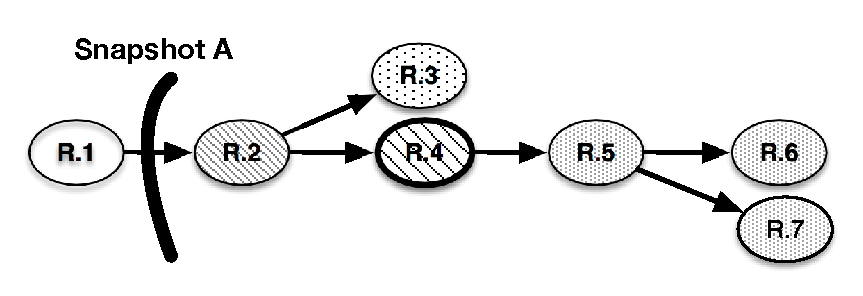
\includegraphics[width=0.7\linewidth]{images/selectiveDependency_paper}
  \caption{{Dependency graph:} $R.1$ precedes snapshot $A$; $R.3$ depends on $R.2$, which is replayed to get the read values; $R.4$ is a malicious request; $R.5,R.6,R.7$ are tainted.}
  \label{fig:selectiveGraph}
\end{figure}


\subsection{Consistency}
\label{sec:recovery:consistency}

An important aspect of a recovery system like Shuttle is the application consistency seen by users. For instance, if a user does an action based on data written by a malicious action, which result of the user action replay is consistent? Since users have a non-deterministic behavior, they may have to be notified if a recovery took place and their data was modified.

Shuttle does not execute requests that returned an error in the first execution. Similarly to other works in the area \cite{undoForOperators}, we assume that these cases were compensated by the user when they happened. As only requests that did not return an error are replayed, Shuttle considers an inconsistency when a request returns an error or a response is different during replay. Shuttle provides the following API for the application programmer to define how inconsistencies are dealt with (Shuttle calls these functions in case they are defined by the tenant):

\begin{enumerate}
  \item \textit{preRecover():} invoked before the beginning of the recovery process.
  \item \textit{handleInconstency(request, previous response, new response, previous keys, new keys, action):} invoked when there is an inconsistency.
  \item \textit{postRecover(statistics, old version, new version):} invoked after the end of the recovery process.
\end{enumerate}

The first function allows tenants to perform a set of actions before the beginning of the recovery process, such as notifying the operations team or taking a new snapshot. 
The second function takes as input the operation that caused the inconsistency as well as the response and keys accessed during the normal execution and during the recovery process. It also takes as argument the action to take. Currently we consider three possible actions: 1) ignore the inconsistency; 2) notify the user of the inconsistency; 3) execute another request. 
Using the \textit{postRecover} function, the tenant has access not only to the statistics of the recovery process but also to an interface to compare the database values before and after the recovery process and the application responses, before exposing the data to the users. 




\subsection{Instance Rejuvenation}
\label{sec:recovery:instance_rejuventaion}
Attackers may exploit system vulnerabilities to tamper application server or database instances, affecting the application integrity or availability. Shuttle interacts with the \ac{PaaS} controller to rejuvenate instances when they are compromised. This process terminates the instances and launches new ones. The PaaS controller initializes the new instances with updated machine images and deploys an updated version of the application code, which may include updates to fix discovered flaws or prevent future intrusions.

We assume new instances to be intrusion-free as the image can be updated to fix previous flaws and their persistent state is renewed. Instances can be launched in a remote site to recover from catastrophic disasters \cite{cloud-disaster}. Tenants are responsible for ensuring that request dependencies remain correct and the updated version API is compatible, or for providing a script to update each request to the new API. Moreover, the selected snapshot has to be consistent according to the updated version specification or every request executed since the application's begin shall be replayed.

This process can be used in a proactive manner to renew instances to remove unknown intrusions \LONG{cite{Castro2002}}\cite{Sousa2010} or to test new application versions to compare its results against the previous version, using the branching mechanism (Section \ref{sec:recovery:runtime_recovery}).


\subsection{Recovery in Runtime}
\label{sec:recovery:runtime_recovery}
Shuttle is capable of doing recovery in runtime, i.e., without making the application unavailable during the recovery period. To do so, each recovery process is considered to be a new branch, a model inspired in versioning systems such as \emph{git} \cite{git}. A \emph{branch} is a sequence of snapshots (akin to commits in \emph{git}). Figure \ref{fig:branches} presents an example with 2 branches and 4 snapshots.

\begin{SCfigure}
  \centering
  \includegraphics[width=30mm]{images/branches_paper}
  \caption{\footnotesize{Tree model:} 2 branches and 4 snapshots: branch 1 contains snapshots A,B,C; Branch 2 contains snapshots A,B,D.}   \label{fig:branches}
\end{SCfigure}

Each recovery process creates a new branch forking a previous snapshot chosen by the tenant, either explicitly or implicitly (by indicating the initial intrusion instant, selecting implicitly the preceding snapshot). Incoming user requests access only the data of the previous branch keeping the application available, while replayed requests access the created branch without compromising the availability of the application. In addiction, tenants can use the branching mechanism to test their intrusion recovery procedures in background, i.e, without exposing users to test issues.

Since tenants can select previous snapshots, we define a branch as a sequence of non-tampered snapshots, named \emph{branch path}. For instance, the snapshots $A,B,D$ compose  branch 2 in the figure. Every database instance knows the \emph{branch path} of the previous branch and the newly created branch in use by the requests being replayed.

Since a novel data item version is created only when the data item is written for the first time during each snapshot, the data item may not have a version for each snapshot (Section \ref{sec:architecture:snapshot}). Therefore, the version \DIFdelbegin \DIFdel{to }\DIFdelend accessed by an operation is defined using the branch path and the \emph{version list} of the data item: operations read the latest version present in the \emph{version list} and in the \emph{branch path} and write the latest version in the branch path. A new version is added to the version list on the first \DIFdelbegin \DIFdel{key }\DIFdelend access to each data item during the replay. This mechanism allows mapping the request to the correct version. Since the \emph{version list} keeps a pointer to the latest version and this reference is updated, the complexity of getting the correct version is $O(1)$. 

At recovery time, the manager sends the new \emph{branch path} to every database instance. The new incoming users access the, perhaps corrupted, old branch while the requests being replaced access the new branch. Therefore, the application remains online, perhaps with a degraded behavior, without exposing downtime to users.

At some point, when the recovery is finishing, the user requests have to start being issued to the new branch. To do so, after replaying the requests, the proxy flag \emph{restraining} is set and every new request is marked with the \emph{restrain} flag. Database accesses marked with \emph{restrain} are delayed. After replaying the requests retrieved during the recovery process, the proxy sets the new branch in the subfield \emph{branch} of \ac{SRD} of the new requests, the \emph{restrain} flag is disabled and the database nodes are notified to proceed the accesses. This mechanism delays the processing of some requests, but this has typically a duration of seconds, compared with a recovery process that may take many minutes or even hours.

\section{Evaluation}
\label{sec:evaluation}


In order to evaluate our approach, we integrated a Shuttle prototype with AppScale and Voldemort. AppScale \cite{Appscale} is an open-source version of Google App Engine. Voldemort \cite{Kreps} is an open source implementation of Dynamo \cite{Decandia2007}, developed and in use by LinkedIn. Shuttle’s prototype has been developed in Java (1400 lines of code for the proxy, 1800 for the manager, 300 for the interceptor, 900 for the replay instances and 1800 for the database proxy).


\subsection{Application Example: Ask}
\label{sec:evaluation:app}

To evaluate Shuttle we developed a \acf{QA} web application for \ac{PaaS} inspired on Stack Exchange\footnote{http://stackexchange.com} (1700 lines of code). The application represents a generic web application that accepts requests and stores the persistent state in  Voldemort. Its implementation is independent of Shuttle, i.e., Shuttle does not require the application to be modified. 

The application semantics implies the following dependencies: a) questions are independent among them; b) answers depend on previous answers and on votes to the same question; c) comments depend on the commented answer; d) votes depend on the answer they vote on. We selected subsets of a dump of the Stack Exchange database to simulate real-world requests.\footnote{Available at: https://archive.org/details/stackexchange} 

\subsection{Accuracy}
\label{sec:evaluation:accuracy}

We evaluate Shuttle's ability to correctly recover applications in different scenarios. We consider three classes of intrusion scenarios: malicious requests, software vulnerabilities and external channels (e.g., SSH connections). The selected data subset contains 100 000 requests originally performed from 31 July until 12 Sep.~2008: 6992 questions, 28993 answers, 2220 comments, 61795 votes\DIFdelbegin \DIFdel{and 3062 tags}\DIFdelend \DIFaddbegin \DIFadd{\LONG{ and 3062 tags}}\DIFaddend . Requests were sorted per date, establishing 92 939 dependencies.


At intrusion moment, Sep.~2nd, the database contains 4338 questions, 18286 answers, 422 comments and 38334 votes (61380 requests). The attack is detected in Sep.~12th, assuming a pessimistic delay of 10 days. During this period, the application executed 38 620 requests. Table \ref{tab:accuracy} presents a summary of the accuracy tests. It contains the number of data items tampered by the intrusion (\emph{\#intrusion}) and the number of user requests that read data items written by  tainted requests or malicious requests (without considering the intrusion requests). Recovery using \textit{full replay} requires to replay every request from the latest snapshot before the intrusion instant until the detection instant: in this example at least 38 620 requests (\emph{\#replayed (fr)}). Selective replay only re-executes tainted requests, unless some data item versions need to be recreated. On the worst case, the system does not contain any snapshot and every data read by the tainted requests shall be recreated (\emph{\#replayed (sr)}). 

\begin{table}
\footnotesize
\begin{tabular}{l|rrrr}
    & \#intrusion & \#tainted & \#replayed (sr)     & \#replayed (fr) \\ \hline
1a       & 110          & 0          & $[0, 605]$   & $> 38 620$  \\
1b       & 58           & 14         & $[0, 379]$   & $> 38 620$  \\
1c       & 48           & 52         & $[0, 253]$   & $> 38 620$  \\
2a       & 4 338        & 0          &  -           & $> 38 620$  \\
2b       & 18 286       & 1 278      &  -           & $> 38 620$  \\
3        & 2 000        & -          &  -           & $> 38 620$  \\
\end{tabular}
  \caption{Number of requests replayed during the recovery process.}
  \label{tab:accuracy}
  \vspace{-5mm}
\end{table}

\textbf{Malicious Requests.} 
 In the first class of scenarios, we consider three  cases in which an attacker has stolen an user credential, then: a) deleted every question created by the user; b) deleted every user answer; or c) modified every user answer.

\textit{1a)} The attacker deletes the user's 4 questions, performing 4 delete requests that remove 106 associated comments and answers. The tenant identifies the malicious requests through the user session and selects a snapshot previous to the intrusion instant. Users cannot access deleted questions, so no request is tainted. If Shuttle has a snapshot containing the deleted questions, then \textit{selective replay} does not need to replay any request and merges the deleted questions on the current system state. If the latest snapshot is previous to the creation of the 4 questions, then \textit{selective replay} replays 605 requests to recreate the deleted questions, their answers and votes. The result is merged with the current branch, rebuilding the deleted questions. 

\textit{1b)} Deleting the user's 48 answers implies that 58 data items are deleted and 14 answers and comments are tainted as they execute after the intrusion instant answering and voting without knowing some answers. If a snapshot containing the user answers exists, then the \textit{selective replay} approach replays only 14 tainted answers and comments. Otherwise, it replays 379 requests: the total number of requests to recreate the tainted questions and then merge the result.


\textit{1c)} 48 data items are modified while 52 requests are tainted because the users replays, votes and comments the modified questions after the intrusion instant. For recovery, the 52 tainted requests shall be replayed. If Shuttle does not have a snapshot containing the questions, then 253 requests have to be replayed to recreate them. 

\textbf{Software vulnerability.}
On the second class, we evaluate intrusion scenarios where software flaws allow attackers to modify the database without authorization. For instance, a code update added a flaw that allows SQL injection. We consider two independent scenarios where the attacker: a) deleted every question; b) deleted every answer.

In \textit{2a)}, the deleting of every question removes 4 338 data items. In \textit{2b)}, the questions are preserved but 1 278 answers, votes and comments are tainted as the user did not see the deleted answers.
Instead of identifying the requests that explored the vulnerability, the tenant patches the code to remove the application vulnerability. Tenants use the instance rejuvenation mechanism to shutdown current application containers and deploy new application version. After, they use the \textit{full replay} to repeat all requests since the beginning of usage of the software version with the flaw. Requests that explored the vulnerability fail to execute and a consistent application state is recovered.



\textbf{External channel.}
On the third class, we consider a case where the proxy does not log the attacker actions. The attacker might use, for example, a SSH account created exploiting the Shellsock vulnerability. The attacker stolen the database credentials and modified at least 2000 data items. Since these database operations are not logged, the dependencies are not established and the number of tainted requests is unknown. However, even without logging the malicious actions, Shuttle recovers the application by loading a database snapshot previous to the estimated intrusion instant (Sep.~2nd) and performing \textit{full replay}. The attack effects are removed because Shuttle loads a database snapshot instead of undoing every operation. As the malicious actions were not logged, they are not replayed and Shuttle recovers the application consistency.


The number of requests to replay is defined by the snapshot instant: on \textit{full replay} Shuttle replays all requests performed after the intrusion instant, while on \textit{selective replay} Shuttle replays the requests necessary to read the values of the entries before the intrusion and the tainted requests. While  \textit{selective replay} seems to have a big advantage comparing with  \textit{full replay}, which performs, in these scenarios, at least 38 620 requests, some applications have more dependencies thus the number of tainted requests is bigger. For instance, if the order between questions with the same tag is considered as a dependency, the number of dependencies rises from 92 939 to 109 118 and the number of independent clusters decreases from 6992 to 56. 


\subsection{Performance}
\label{sec:evaluation:performance}

We evaluate Shuttle's performance considering the throughput of the application, the size of the logs and the recovery time. We also estimate the cost of deployment of Shuttle on a public cloud provider, \acf{AWS}. We run 6 \ac{AWS} \textit{c3.xlarge} instances (14 ECUs, 4 vCPUs, 2.8 GHz, Intel Xeon E5-2680v2, 7.5 GB of memory, 2 x 40 GB storage capacity) connected by gigabit ethernet (780Mbps measured with \emph{iperf}, 0.176ms round-trip time measured with \emph{ping}). We use one client, one instance with Shuttle proxy and a load balancer (HAProxy), three WildFly (formerly JBoss) application servers and one Voldemort database. We consider a large data sample from the data of Stack Exchange with 50 000 requests (1432 questions, 3399 answers, 8335 comments, 36834 votes, 950 000 question views). We do not consider a particular scenario or replay scheme (full/selective), but define instead the number of requests recovered per experiment.

\textbf{Performance overhead.}
We evaluate the overhead of Shuttle by measuring the throughput of the \textit{Ask} application with and without Shuttle (Table \ref{tab:throughput}). We considered two workloads: (A) 50\% reads, 50\% writes;  (B)  95\% reads, 5\% writes. Write operations insert questions, answers, comments and votes of the data sample, while the read operations access the latest inserted questions. Table \ref{tab:throughput} shows that Shuttle imposes an overhead of 13-20\%, which seems reasonable considering its benefits. We believe the main cause of overhead is the current proxy \DIFaddbegin \DIFadd{implementation}\DIFaddend , which is not very efficient. The current version written in Java performs considerably better than a previous version in Python, but we expect to improve it further by rewriting it in C.

\begin{table}
\footnotesize
\begin{tabular}{l|rr}
                       &  Workload A                    & Workload B  \\ \hline
Shuttle                &  6325 ops/sec [5.78 ms]        &  15346 ops/sec [3.62 ms]  \\
No Shuttle             &  7148 ops/sec [5.07 ms]        &  17821 ops/sec [3.01 ms]  \\
overhead               &  13\% [14\%]                    & 16\% [20\%] \\
\end{tabular}
\caption{Overhead in throughput (ops/sec) and response latency (ms).}
\label{tab:throughput}
\vspace{-3mm}
\end{table}

In order to measure Shuttle's overhead on the database accesses, we used the \acf{YCSB} framework \cite{ycsb}. We considered two workloads: (A)  50\% reads, 50\% updates; (B)  95\% reads, 5\% updates. Operations access 1KB records following a Zipfian distribution (Figure \ref{fig:database_overhead}). Results show Shuttle has small impact on the latency of database accesses. 

\begin{figure}[tbh]
\vspace{-6mm}
\hspace*{-0.5cm}
  \LARGE
  \mbox{
      \subfloat[][Workload A - update \label{fig:database:a:update}]{
      \hspace{-0.5cm}
        \resizebox{4.5cm}{!}{\begingroup
  \makeatletter
  \providecommand\color[2][]{    \GenericError{(gnuplot) \space\space\space\@spaces}{      Package color not loaded in conjunction with
      terminal option `colourtext'    }{See the gnuplot documentation for explanation.    }{Either use 'blacktext' in gnuplot or load the package
      color.sty in LaTeX.}    \renewcommand\color[2][]{}  }  \providecommand\includegraphics[2][]{    \GenericError{(gnuplot) \space\space\space\@spaces}{      Package graphicx or graphics not loaded    }{See the gnuplot documentation for explanation.    }{The gnuplot epslatex terminal needs graphicx.sty or graphics.sty.}    \renewcommand\includegraphics[2][]{}  }  \providecommand\rotatebox[2]{#2}  \@ifundefined{ifGPcolor}{    \newif\ifGPcolor
    \GPcolorfalse
  }{}  \@ifundefined{ifGPblacktext}{    \newif\ifGPblacktext
    \GPblacktexttrue
  }{}    \let\gplgaddtomacro\g@addto@macro
    \gdef\gplbacktext{}  \gdef\gplfronttext{}  \makeatother
  \ifGPblacktext
        \def\colorrgb#1{}    \def\colorgray#1{}  \else
        \ifGPcolor
      \def\colorrgb#1{\color[rgb]{#1}}      \def\colorgray#1{\color[gray]{#1}}      \expandafter\def\csname LTw\endcsname{\color{white}}      \expandafter\def\csname LTb\endcsname{\color{black}}      \expandafter\def\csname LTa\endcsname{\color{black}}      \expandafter\def\csname LT0\endcsname{\color[rgb]{1,0,0}}      \expandafter\def\csname LT1\endcsname{\color[rgb]{0,1,0}}      \expandafter\def\csname LT2\endcsname{\color[rgb]{0,0,1}}      \expandafter\def\csname LT3\endcsname{\color[rgb]{1,0,1}}      \expandafter\def\csname LT4\endcsname{\color[rgb]{0,1,1}}      \expandafter\def\csname LT5\endcsname{\color[rgb]{1,1,0}}      \expandafter\def\csname LT6\endcsname{\color[rgb]{0,0,0}}      \expandafter\def\csname LT7\endcsname{\color[rgb]{1,0.3,0}}      \expandafter\def\csname LT8\endcsname{\color[rgb]{0.5,0.5,0.5}}    \else
            \def\colorrgb#1{\color{black}}      \def\colorgray#1{\color[gray]{#1}}      \expandafter\def\csname LTw\endcsname{\color{white}}      \expandafter\def\csname LTb\endcsname{\color{black}}      \expandafter\def\csname LTa\endcsname{\color{black}}      \expandafter\def\csname LT0\endcsname{\color{black}}      \expandafter\def\csname LT1\endcsname{\color{black}}      \expandafter\def\csname LT2\endcsname{\color{black}}      \expandafter\def\csname LT3\endcsname{\color{black}}      \expandafter\def\csname LT4\endcsname{\color{black}}      \expandafter\def\csname LT5\endcsname{\color{black}}      \expandafter\def\csname LT6\endcsname{\color{black}}      \expandafter\def\csname LT7\endcsname{\color{black}}      \expandafter\def\csname LT8\endcsname{\color{black}}    \fi
  \fi
  \setlength{\unitlength}{0.0500bp}  \begin{picture}(7200.00,5040.00)    \gplgaddtomacro\gplbacktext{      \csname LTb\endcsname      \put(1078,704){\makebox(0,0)[r]{\strut{} 0}}      \put(1078,1629){\makebox(0,0)[r]{\strut{} 500}}      \put(1078,2554){\makebox(0,0)[r]{\strut{} 1000}}      \put(1078,3480){\makebox(0,0)[r]{\strut{} 1500}}      \put(1078,4405){\makebox(0,0)[r]{\strut{} 2000}}      \put(1210,484){\makebox(0,0){\strut{} 5}}      \put(2009,484){\makebox(0,0){\strut{} 10}}      \put(2808,484){\makebox(0,0){\strut{} 15}}      \put(3607,484){\makebox(0,0){\strut{} 20}}      \put(4406,484){\makebox(0,0){\strut{} 25}}      \put(5205,484){\makebox(0,0){\strut{} 30}}      \put(6004,484){\makebox(0,0){\strut{} 35}}      \put(6803,484){\makebox(0,0){\strut{} 40}}      \put(176,2739){\rotatebox{-270}{\makebox(0,0){\strut{}Update latency (us)}}}      \put(4006,154){\makebox(0,0){\strut{}Throughput (thousand ops/sec)}}    }    \gplgaddtomacro\gplfronttext{      \csname LTb\endcsname      \put(5816,1416){\makebox(0,0)[r]{\strut{}Shuttle}}      \csname LTb\endcsname      \put(5816,1042){\makebox(0,0)[r]{\strut{}No Shuttle}}    }    \gplbacktext
    \put(0,0){\includegraphics{graphs/database/a_update}}    \gplfronttext
  \end{picture}\endgroup
}
      }
      \subfloat[][Workload B - read \label{fig:database:b:read}]{
      \hspace{-0.7cm}
        \resizebox{4.5cm}{!}{\begingroup
  \makeatletter
  \providecommand\color[2][]{    \GenericError{(gnuplot) \space\space\space\@spaces}{      Package color not loaded in conjunction with
      terminal option `colourtext'    }{See the gnuplot documentation for explanation.    }{Either use 'blacktext' in gnuplot or load the package
      color.sty in LaTeX.}    \renewcommand\color[2][]{}  }  \providecommand\includegraphics[2][]{    \GenericError{(gnuplot) \space\space\space\@spaces}{      Package graphicx or graphics not loaded    }{See the gnuplot documentation for explanation.    }{The gnuplot epslatex terminal needs graphicx.sty or graphics.sty.}    \renewcommand\includegraphics[2][]{}  }  \providecommand\rotatebox[2]{#2}  \@ifundefined{ifGPcolor}{    \newif\ifGPcolor
    \GPcolorfalse
  }{}  \@ifundefined{ifGPblacktext}{    \newif\ifGPblacktext
    \GPblacktexttrue
  }{}    \let\gplgaddtomacro\g@addto@macro
    \gdef\gplbacktext{}  \gdef\gplfronttext{}  \makeatother
  \ifGPblacktext
        \def\colorrgb#1{}    \def\colorgray#1{}  \else
        \ifGPcolor
      \def\colorrgb#1{\color[rgb]{#1}}      \def\colorgray#1{\color[gray]{#1}}      \expandafter\def\csname LTw\endcsname{\color{white}}      \expandafter\def\csname LTb\endcsname{\color{black}}      \expandafter\def\csname LTa\endcsname{\color{black}}      \expandafter\def\csname LT0\endcsname{\color[rgb]{1,0,0}}      \expandafter\def\csname LT1\endcsname{\color[rgb]{0,1,0}}      \expandafter\def\csname LT2\endcsname{\color[rgb]{0,0,1}}      \expandafter\def\csname LT3\endcsname{\color[rgb]{1,0,1}}      \expandafter\def\csname LT4\endcsname{\color[rgb]{0,1,1}}      \expandafter\def\csname LT5\endcsname{\color[rgb]{1,1,0}}      \expandafter\def\csname LT6\endcsname{\color[rgb]{0,0,0}}      \expandafter\def\csname LT7\endcsname{\color[rgb]{1,0.3,0}}      \expandafter\def\csname LT8\endcsname{\color[rgb]{0.5,0.5,0.5}}    \else
            \def\colorrgb#1{\color{black}}      \def\colorgray#1{\color[gray]{#1}}      \expandafter\def\csname LTw\endcsname{\color{white}}      \expandafter\def\csname LTb\endcsname{\color{black}}      \expandafter\def\csname LTa\endcsname{\color{black}}      \expandafter\def\csname LT0\endcsname{\color{black}}      \expandafter\def\csname LT1\endcsname{\color{black}}      \expandafter\def\csname LT2\endcsname{\color{black}}      \expandafter\def\csname LT3\endcsname{\color{black}}      \expandafter\def\csname LT4\endcsname{\color{black}}      \expandafter\def\csname LT5\endcsname{\color{black}}      \expandafter\def\csname LT6\endcsname{\color{black}}      \expandafter\def\csname LT7\endcsname{\color{black}}      \expandafter\def\csname LT8\endcsname{\color{black}}    \fi
  \fi
  \setlength{\unitlength}{0.0500bp}  \begin{picture}(7200.00,5040.00)    \gplgaddtomacro\gplbacktext{      \csname LTb\endcsname      \put(1078,704){\makebox(0,0)[r]{\strut{} 0}}      \put(1078,1629){\makebox(0,0)[r]{\strut{} 500}}      \put(1078,2554){\makebox(0,0)[r]{\strut{} 1000}}      \put(1078,3480){\makebox(0,0)[r]{\strut{} 1500}}      \put(1078,4405){\makebox(0,0)[r]{\strut{} 2000}}      \put(1210,484){\makebox(0,0){\strut{} 5}}      \put(2009,484){\makebox(0,0){\strut{} 10}}      \put(2808,484){\makebox(0,0){\strut{} 15}}      \put(3607,484){\makebox(0,0){\strut{} 20}}      \put(4406,484){\makebox(0,0){\strut{} 25}}      \put(5205,484){\makebox(0,0){\strut{} 30}}      \put(6004,484){\makebox(0,0){\strut{} 35}}      \put(6803,484){\makebox(0,0){\strut{} 40}}      \put(176,2739){\rotatebox{-270}{\makebox(0,0){\strut{}Read latency (us)}}}      \put(4006,154){\makebox(0,0){\strut{}Throughput (thousand ops/sec)}}    }    \gplgaddtomacro\gplfronttext{      \csname LTb\endcsname      \put(5816,1416){\makebox(0,0)[r]{\strut{}Shuttle}}      \csname LTb\endcsname      \put(5816,1042){\makebox(0,0)[r]{\strut{}No Shuttle}}    }    \gplbacktext
    \put(0,0){\includegraphics{graphs/database/b_read}}    \gplfronttext
  \end{picture}\endgroup
}
      }
  }
  \caption{Performance overhead on database.}
  \vspace{-2mm}
  \label{fig:database_overhead}
\end{figure}


\textbf{Recovery.}
We measured the recovery time using Shuttle to replay the sample of 1 million requests. While serial replay (1 cluster) takes approximately 30 minutes (1717s), recovery with clusters takes only 9 minutes (544s) (Figure \ref{fig:recovery_times}).

We measured the recovery period with different numbers of instances on clustered mode (Figure \ref{fig:scalability}). The figure shows that Shuttle is scalable, in the sense that adding more servers allow reducing the time of recovery (3 servers allowed recovery in half the time of 1, $\sim$750s versus $\sim$400s). 

\begin{figure}[tbh]
\vspace{-5mm}
  \LARGE
  \mbox{
      \subfloat[][Recovery time \label{fig:recovery_times}]{
      \hspace{-0.5cm}
        \resizebox{4.5cm}{!}{\begingroup
  \makeatletter
  \providecommand\color[2][]{    \GenericError{(gnuplot) \space\space\space\@spaces}{      Package color not loaded in conjunction with
      terminal option `colourtext'    }{See the gnuplot documentation for explanation.    }{Either use 'blacktext' in gnuplot or load the package
      color.sty in LaTeX.}    \renewcommand\color[2][]{}  }  \providecommand\includegraphics[2][]{    \GenericError{(gnuplot) \space\space\space\@spaces}{      Package graphicx or graphics not loaded    }{See the gnuplot documentation for explanation.    }{The gnuplot epslatex terminal needs graphicx.sty or graphics.sty.}    \renewcommand\includegraphics[2][]{}  }  \providecommand\rotatebox[2]{#2}  \@ifundefined{ifGPcolor}{    \newif\ifGPcolor
    \GPcolorfalse
  }{}  \@ifundefined{ifGPblacktext}{    \newif\ifGPblacktext
    \GPblacktexttrue
  }{}    \let\gplgaddtomacro\g@addto@macro
    \gdef\gplbacktext{}  \gdef\gplfronttext{}  \makeatother
  \ifGPblacktext
        \def\colorrgb#1{}    \def\colorgray#1{}  \else
        \ifGPcolor
      \def\colorrgb#1{\color[rgb]{#1}}      \def\colorgray#1{\color[gray]{#1}}      \expandafter\def\csname LTw\endcsname{\color{white}}      \expandafter\def\csname LTb\endcsname{\color{black}}      \expandafter\def\csname LTa\endcsname{\color{black}}      \expandafter\def\csname LT0\endcsname{\color[rgb]{1,0,0}}      \expandafter\def\csname LT1\endcsname{\color[rgb]{0,1,0}}      \expandafter\def\csname LT2\endcsname{\color[rgb]{0,0,1}}      \expandafter\def\csname LT3\endcsname{\color[rgb]{1,0,1}}      \expandafter\def\csname LT4\endcsname{\color[rgb]{0,1,1}}      \expandafter\def\csname LT5\endcsname{\color[rgb]{1,1,0}}      \expandafter\def\csname LT6\endcsname{\color[rgb]{0,0,0}}      \expandafter\def\csname LT7\endcsname{\color[rgb]{1,0.3,0}}      \expandafter\def\csname LT8\endcsname{\color[rgb]{0.5,0.5,0.5}}    \else
            \def\colorrgb#1{\color{black}}      \def\colorgray#1{\color[gray]{#1}}      \expandafter\def\csname LTw\endcsname{\color{white}}      \expandafter\def\csname LTb\endcsname{\color{black}}      \expandafter\def\csname LTa\endcsname{\color{black}}      \expandafter\def\csname LT0\endcsname{\color{black}}      \expandafter\def\csname LT1\endcsname{\color{black}}      \expandafter\def\csname LT2\endcsname{\color{black}}      \expandafter\def\csname LT3\endcsname{\color{black}}      \expandafter\def\csname LT4\endcsname{\color{black}}      \expandafter\def\csname LT5\endcsname{\color{black}}      \expandafter\def\csname LT6\endcsname{\color{black}}      \expandafter\def\csname LT7\endcsname{\color{black}}      \expandafter\def\csname LT8\endcsname{\color{black}}    \fi
  \fi
  \setlength{\unitlength}{0.0500bp}  \begin{picture}(7200.00,5040.00)    \gplgaddtomacro\gplbacktext{      \csname LTb\endcsname      \put(1078,704){\makebox(0,0)[r]{\strut{} 0}}      \put(1078,1518){\makebox(0,0)[r]{\strut{} 500}}      \put(1078,2332){\makebox(0,0)[r]{\strut{} 1000}}      \put(1078,3147){\makebox(0,0)[r]{\strut{} 1500}}      \put(1078,3961){\makebox(0,0)[r]{\strut{} 2000}}      \put(1078,4775){\makebox(0,0)[r]{\strut{} 2500}}      \put(1210,484){\makebox(0,0){\strut{}00:00}}      \put(2142,484){\makebox(0,0){\strut{}05:00}}      \put(3074,484){\makebox(0,0){\strut{}10:00}}      \put(4007,484){\makebox(0,0){\strut{}15:00}}      \put(4939,484){\makebox(0,0){\strut{}20:00}}      \put(5871,484){\makebox(0,0){\strut{}25:00}}      \put(6803,484){\makebox(0,0){\strut{}30:00}}      \put(176,2739){\rotatebox{-270}{\makebox(0,0){\strut{}Requests per second}}}      \put(4006,154){\makebox(0,0){\strut{}Time (minutes:seconds)}}    }    \gplgaddtomacro\gplfronttext{      \csname LTb\endcsname      \put(5816,4481){\makebox(0,0)[r]{\strut{}serial replay}}      \csname LTb\endcsname      \put(5816,4195){\makebox(0,0)[r]{\strut{}clustered replay}}    }    \gplbacktext
    \put(0,0){\includegraphics{graphs/replay/grafico_paper}}    \gplfronttext
  \end{picture}\endgroup
}
      }
      \subfloat[][Scalability \label{fig:scalability}]{
      \hspace{-0.7cm}
        \resizebox{4.5cm}{!}{\begingroup
  \makeatletter
  \providecommand\color[2][]{    \GenericError{(gnuplot) \space\space\space\@spaces}{      Package color not loaded in conjunction with
      terminal option `colourtext'    }{See the gnuplot documentation for explanation.    }{Either use 'blacktext' in gnuplot or load the package
      color.sty in LaTeX.}    \renewcommand\color[2][]{}  }  \providecommand\includegraphics[2][]{    \GenericError{(gnuplot) \space\space\space\@spaces}{      Package graphicx or graphics not loaded    }{See the gnuplot documentation for explanation.    }{The gnuplot epslatex terminal needs graphicx.sty or graphics.sty.}    \renewcommand\includegraphics[2][]{}  }  \providecommand\rotatebox[2]{#2}  \@ifundefined{ifGPcolor}{    \newif\ifGPcolor
    \GPcolorfalse
  }{}  \@ifundefined{ifGPblacktext}{    \newif\ifGPblacktext
    \GPblacktexttrue
  }{}    \let\gplgaddtomacro\g@addto@macro
    \gdef\gplbacktext{}  \gdef\gplfronttext{}  \makeatother
  \ifGPblacktext
        \def\colorrgb#1{}    \def\colorgray#1{}  \else
        \ifGPcolor
      \def\colorrgb#1{\color[rgb]{#1}}      \def\colorgray#1{\color[gray]{#1}}      \expandafter\def\csname LTw\endcsname{\color{white}}      \expandafter\def\csname LTb\endcsname{\color{black}}      \expandafter\def\csname LTa\endcsname{\color{black}}      \expandafter\def\csname LT0\endcsname{\color[rgb]{1,0,0}}      \expandafter\def\csname LT1\endcsname{\color[rgb]{0,1,0}}      \expandafter\def\csname LT2\endcsname{\color[rgb]{0,0,1}}      \expandafter\def\csname LT3\endcsname{\color[rgb]{1,0,1}}      \expandafter\def\csname LT4\endcsname{\color[rgb]{0,1,1}}      \expandafter\def\csname LT5\endcsname{\color[rgb]{1,1,0}}      \expandafter\def\csname LT6\endcsname{\color[rgb]{0,0,0}}      \expandafter\def\csname LT7\endcsname{\color[rgb]{1,0.3,0}}      \expandafter\def\csname LT8\endcsname{\color[rgb]{0.5,0.5,0.5}}    \else
            \def\colorrgb#1{\color{black}}      \def\colorgray#1{\color[gray]{#1}}      \expandafter\def\csname LTw\endcsname{\color{white}}      \expandafter\def\csname LTb\endcsname{\color{black}}      \expandafter\def\csname LTa\endcsname{\color{black}}      \expandafter\def\csname LT0\endcsname{\color{black}}      \expandafter\def\csname LT1\endcsname{\color{black}}      \expandafter\def\csname LT2\endcsname{\color{black}}      \expandafter\def\csname LT3\endcsname{\color{black}}      \expandafter\def\csname LT4\endcsname{\color{black}}      \expandafter\def\csname LT5\endcsname{\color{black}}      \expandafter\def\csname LT6\endcsname{\color{black}}      \expandafter\def\csname LT7\endcsname{\color{black}}      \expandafter\def\csname LT8\endcsname{\color{black}}    \fi
  \fi
  \setlength{\unitlength}{0.0500bp}  \begin{picture}(7200.00,5040.00)    \gplgaddtomacro\gplbacktext{      \csname LTb\endcsname      \put(946,704){\makebox(0,0)[r]{\strut{} 0}}      \put(946,1156){\makebox(0,0)[r]{\strut{} 100}}      \put(946,1609){\makebox(0,0)[r]{\strut{} 200}}      \put(946,2061){\makebox(0,0)[r]{\strut{} 300}}      \put(946,2513){\makebox(0,0)[r]{\strut{} 400}}      \put(946,2966){\makebox(0,0)[r]{\strut{} 500}}      \put(946,3418){\makebox(0,0)[r]{\strut{} 600}}      \put(946,3870){\makebox(0,0)[r]{\strut{} 700}}      \put(946,4323){\makebox(0,0)[r]{\strut{} 800}}      \put(946,4775){\makebox(0,0)[r]{\strut{} 900}}      \put(1078,484){\makebox(0,0){\strut{} 0}}      \put(1896,484){\makebox(0,0){\strut{} 1}}      \put(2714,484){\makebox(0,0){\strut{} 2}}      \put(3532,484){\makebox(0,0){\strut{} 3}}      \put(4349,484){\makebox(0,0){\strut{} 4}}      \put(5167,484){\makebox(0,0){\strut{} 5}}      \put(5985,484){\makebox(0,0){\strut{} 6}}      \put(6803,484){\makebox(0,0){\strut{} 7}}      \put(176,2739){\rotatebox{-270}{\makebox(0,0){\strut{}Time to recovery (seconds)}}}      \put(3940,154){\makebox(0,0){\strut{}Number of application servers}}    }    \gplgaddtomacro\gplfronttext{      \csname LTb\endcsname      \put(5816,4481){\makebox(0,0)[r]{\strut{}1 replay; 1 database}}    }    \gplbacktext
    \put(0,0){\includegraphics{graphs/scalability/recovery_time_paper}}    \gplfronttext
  \end{picture}\endgroup
}
      }
  }
  \caption{Recovery time and scalability.}
  \vspace{-3mm}
\end{figure}

We measured the duration of the restrain period considering two clients with a constant throughput of 400 requests/sec. The serial replay mode is not capable of fully exploring the application servers so it takes almost one hour to recover (2953s total, 1100s in restrain mode) (Fig. \ref{fig:restrain:serial}). The clustered mode takes 10 minutes (635s), from which the restrain period represents 46 seconds. (Fig. \ref{fig:restrain:clustered}).

\begin{figure}[tbh]
\vspace{-5mm}
  \LARGE
  \mbox{
    \subfloat[][Serial \label{fig:restrain:serial}]{
      \hspace{-0.5cm}
      \resizebox{4.5cm}{!}{\begingroup
  \makeatletter
  \providecommand\color[2][]{    \GenericError{(gnuplot) \space\space\space\@spaces}{      Package color not loaded in conjunction with
      terminal option `colourtext'    }{See the gnuplot documentation for explanation.    }{Either use 'blacktext' in gnuplot or load the package
      color.sty in LaTeX.}    \renewcommand\color[2][]{}  }  \providecommand\includegraphics[2][]{    \GenericError{(gnuplot) \space\space\space\@spaces}{      Package graphicx or graphics not loaded    }{See the gnuplot documentation for explanation.    }{The gnuplot epslatex terminal needs graphicx.sty or graphics.sty.}    \renewcommand\includegraphics[2][]{}  }  \providecommand\rotatebox[2]{#2}  \@ifundefined{ifGPcolor}{    \newif\ifGPcolor
    \GPcolorfalse
  }{}  \@ifundefined{ifGPblacktext}{    \newif\ifGPblacktext
    \GPblacktexttrue
  }{}    \let\gplgaddtomacro\g@addto@macro
    \gdef\gplbacktext{}  \gdef\gplfronttext{}  \makeatother
  \ifGPblacktext
        \def\colorrgb#1{}    \def\colorgray#1{}  \else
        \ifGPcolor
      \def\colorrgb#1{\color[rgb]{#1}}      \def\colorgray#1{\color[gray]{#1}}      \expandafter\def\csname LTw\endcsname{\color{white}}      \expandafter\def\csname LTb\endcsname{\color{black}}      \expandafter\def\csname LTa\endcsname{\color{black}}      \expandafter\def\csname LT0\endcsname{\color[rgb]{1,0,0}}      \expandafter\def\csname LT1\endcsname{\color[rgb]{0,1,0}}      \expandafter\def\csname LT2\endcsname{\color[rgb]{0,0,1}}      \expandafter\def\csname LT3\endcsname{\color[rgb]{1,0,1}}      \expandafter\def\csname LT4\endcsname{\color[rgb]{0,1,1}}      \expandafter\def\csname LT5\endcsname{\color[rgb]{1,1,0}}      \expandafter\def\csname LT6\endcsname{\color[rgb]{0,0,0}}      \expandafter\def\csname LT7\endcsname{\color[rgb]{1,0.3,0}}      \expandafter\def\csname LT8\endcsname{\color[rgb]{0.5,0.5,0.5}}    \else
            \def\colorrgb#1{\color{black}}      \def\colorgray#1{\color[gray]{#1}}      \expandafter\def\csname LTw\endcsname{\color{white}}      \expandafter\def\csname LTb\endcsname{\color{black}}      \expandafter\def\csname LTa\endcsname{\color{black}}      \expandafter\def\csname LT0\endcsname{\color{black}}      \expandafter\def\csname LT1\endcsname{\color{black}}      \expandafter\def\csname LT2\endcsname{\color{black}}      \expandafter\def\csname LT3\endcsname{\color{black}}      \expandafter\def\csname LT4\endcsname{\color{black}}      \expandafter\def\csname LT5\endcsname{\color{black}}      \expandafter\def\csname LT6\endcsname{\color{black}}      \expandafter\def\csname LT7\endcsname{\color{black}}      \expandafter\def\csname LT8\endcsname{\color{black}}    \fi
  \fi
  \setlength{\unitlength}{0.0500bp}  \begin{picture}(7200.00,5040.00)    \gplgaddtomacro\gplbacktext{      \csname LTb\endcsname      \put(1078,704){\makebox(0,0)[r]{\strut{} 0}}      \put(1078,1458){\makebox(0,0)[r]{\strut{} 500}}      \put(1078,2212){\makebox(0,0)[r]{\strut{} 1000}}      \put(1078,2966){\makebox(0,0)[r]{\strut{} 1500}}      \put(1078,3720){\makebox(0,0)[r]{\strut{} 2000}}      \put(1078,4473){\makebox(0,0)[r]{\strut{} 2500}}      \put(1210,484){\makebox(0,0){\strut{}00:00}}      \put(2329,484){\makebox(0,0){\strut{}10:00}}      \put(3447,484){\makebox(0,0){\strut{}20:00}}      \put(4566,484){\makebox(0,0){\strut{}30:00}}      \put(5684,484){\makebox(0,0){\strut{}40:00}}      \put(6803,484){\makebox(0,0){\strut{}50:00}}      \put(176,2739){\rotatebox{-270}{\makebox(0,0){\strut{}Requests per second}}}      \put(4006,154){\makebox(0,0){\strut{}Time (minutes:seconds)}}      \put(4659,2966){\makebox(0,0)[l]{\strut{}Restrain}}    }    \gplgaddtomacro\gplfronttext{      \csname LTb\endcsname      \put(2398,4481){\makebox(0,0)[r]{\strut{}serial}}      \csname LTb\endcsname      \put(2398,4195){\makebox(0,0)[r]{\strut{}client}}    }    \gplbacktext
    \put(0,0){\includegraphics{graphs/restrain/serial_paper}}    \gplfronttext
  \end{picture}\endgroup
}
    }
    \subfloat[][Clustered \label{fig:restrain:clustered}]{
      \hspace{-0.7cm}
      \resizebox{4.5cm}{!}{\begingroup
  \makeatletter
  \providecommand\color[2][]{    \GenericError{(gnuplot) \space\space\space\@spaces}{      Package color not loaded in conjunction with
      terminal option `colourtext'    }{See the gnuplot documentation for explanation.    }{Either use 'blacktext' in gnuplot or load the package
      color.sty in LaTeX.}    \renewcommand\color[2][]{}  }  \providecommand\includegraphics[2][]{    \GenericError{(gnuplot) \space\space\space\@spaces}{      Package graphicx or graphics not loaded    }{See the gnuplot documentation for explanation.    }{The gnuplot epslatex terminal needs graphicx.sty or graphics.sty.}    \renewcommand\includegraphics[2][]{}  }  \providecommand\rotatebox[2]{#2}  \@ifundefined{ifGPcolor}{    \newif\ifGPcolor
    \GPcolorfalse
  }{}  \@ifundefined{ifGPblacktext}{    \newif\ifGPblacktext
    \GPblacktexttrue
  }{}    \let\gplgaddtomacro\g@addto@macro
    \gdef\gplbacktext{}  \gdef\gplfronttext{}  \makeatother
  \ifGPblacktext
        \def\colorrgb#1{}    \def\colorgray#1{}  \else
        \ifGPcolor
      \def\colorrgb#1{\color[rgb]{#1}}      \def\colorgray#1{\color[gray]{#1}}      \expandafter\def\csname LTw\endcsname{\color{white}}      \expandafter\def\csname LTb\endcsname{\color{black}}      \expandafter\def\csname LTa\endcsname{\color{black}}      \expandafter\def\csname LT0\endcsname{\color[rgb]{1,0,0}}      \expandafter\def\csname LT1\endcsname{\color[rgb]{0,1,0}}      \expandafter\def\csname LT2\endcsname{\color[rgb]{0,0,1}}      \expandafter\def\csname LT3\endcsname{\color[rgb]{1,0,1}}      \expandafter\def\csname LT4\endcsname{\color[rgb]{0,1,1}}      \expandafter\def\csname LT5\endcsname{\color[rgb]{1,1,0}}      \expandafter\def\csname LT6\endcsname{\color[rgb]{0,0,0}}      \expandafter\def\csname LT7\endcsname{\color[rgb]{1,0.3,0}}      \expandafter\def\csname LT8\endcsname{\color[rgb]{0.5,0.5,0.5}}    \else
            \def\colorrgb#1{\color{black}}      \def\colorgray#1{\color[gray]{#1}}      \expandafter\def\csname LTw\endcsname{\color{white}}      \expandafter\def\csname LTb\endcsname{\color{black}}      \expandafter\def\csname LTa\endcsname{\color{black}}      \expandafter\def\csname LT0\endcsname{\color{black}}      \expandafter\def\csname LT1\endcsname{\color{black}}      \expandafter\def\csname LT2\endcsname{\color{black}}      \expandafter\def\csname LT3\endcsname{\color{black}}      \expandafter\def\csname LT4\endcsname{\color{black}}      \expandafter\def\csname LT5\endcsname{\color{black}}      \expandafter\def\csname LT6\endcsname{\color{black}}      \expandafter\def\csname LT7\endcsname{\color{black}}      \expandafter\def\csname LT8\endcsname{\color{black}}    \fi
  \fi
  \setlength{\unitlength}{0.0500bp}  \begin{picture}(7200.00,5040.00)    \gplgaddtomacro\gplbacktext{      \csname LTb\endcsname      \put(1078,704){\makebox(0,0)[r]{\strut{} 0}}      \put(1078,1458){\makebox(0,0)[r]{\strut{} 500}}      \put(1078,2212){\makebox(0,0)[r]{\strut{} 1000}}      \put(1078,2966){\makebox(0,0)[r]{\strut{} 1500}}      \put(1078,3720){\makebox(0,0)[r]{\strut{} 2000}}      \put(1078,4473){\makebox(0,0)[r]{\strut{} 2500}}      \put(1210,484){\makebox(0,0){\strut{}00:00}}      \put(2795,484){\makebox(0,0){\strut{}03:00}}      \put(4381,484){\makebox(0,0){\strut{}06:00}}      \put(5966,484){\makebox(0,0){\strut{}09:00}}      \put(176,2739){\rotatebox{-270}{\makebox(0,0){\strut{}Requests per second}}}      \put(4006,154){\makebox(0,0){\strut{}Time (minutes:seconds)}}      \put(5174,4473){\makebox(0,0)[l]{\strut{}Restrain}}    }    \gplgaddtomacro\gplfronttext{      \csname LTb\endcsname      \put(2794,4481){\makebox(0,0)[r]{\strut{}clustered}}      \csname LTb\endcsname      \put(2794,4195){\makebox(0,0)[r]{\strut{}client}}    }    \gplbacktext
    \put(0,0){\includegraphics{graphs/restrain/clustered_paper}}    \gplfronttext
  \end{picture}\endgroup
}
    }
  }
  \caption{Restrain period in serial and clustered recovery (\emph{Restrain} indicates the beggining of the period that ends at the end of the graphic).}
  \vspace{-3mm}
\end{figure}


\textbf{Space overhead.}
We measured the memory and storage overhead of 1 million requests, from which 95\% were requests for reading questions. Table \ref{tab:storage_overhead} presents the size of each component in memory\LONG{footnote{https://code.google.com/p/memory-measurer}}. Requests and keys are stored in the external database while the dependency graph and the accesses are kept in the manager and database instances. No snapshot has been taken and the data is not compressed.
In the current implementation, the \ac{SRD} represents a fixed overhead of 35 bytes per request.

\begin{table}[h]
\centering
\footnotesize
  \begin{tabular}{l|rr}
                & \# objects & size (MB) \\ \hline
  \textbf{Shuttle Storage: }      \\
  Request         & 1 million    & 212       \\    Response        & 1 million    & 8 967     \\    Start/end timestamps      & 2 million    & 16        \\    Keys            & 137 million  & 488       \\    Total           &              & 9 684     \\    \textbf{Database node:}        &           \\
  Version List    &  14 593      &  1.4       \\   Operation list  &  9 million   &  277       \\   Total           &              & 282 \\   \textbf{Manager:} & & \\ 
  Graph           & 1 million    & 718 \\    \end{tabular}            
\caption{Storage used by Shuttle  \DIFaddbeginFL \DIFaddFL{(1 million requests)}\DIFaddendFL .}
\label{tab:storage_overhead}
\vspace{-5mm}
\end{table}

The main overhead are the responses, as we are storing them complete (full HTML pages), although  Shuttle has to store them only if the tenant uses the API to solve inconsistencies (Section \ref{sec:recovery:consistency}). The size of the list of keys accessed by the request depends on the key length and the number of keys accessed. Each access implies an overhead of 13 bytes to record the request ID and the operation type in the version list. The snapshot does not impact the throughput but requires to track the new version, which implies a storage overhead of 10 bytes for each data item when it is written by the first time after a snapshot. This overhead can be reduced implementing the version list as a bitmap. The total database storage overhead encompasses synchronization mechanisms. Since the dependency graph is implemented as a double-linked graph, each entry in the dependency graph has 765 bytes to store not only the start/end instant of the request but also the requests which this request depends from and to (10 on average). Serialization mechanisms and compression techniques can reduce the storage overhead. For instance, Cassandra's \emph{lz4}\LONG{cite{lz4}} reduces the size of the Shuttle Storage on disk to 4.9 GB.


\textbf{Monetary cost.}
Since the replay instances are allocated on demand and paid per use, the cost of Shuttle is dominated by the storage. 
For instance, consider the extreme case of 20 million requests/day with overhead proportional to the values in Table \ref{tab:storage_overhead} to show that the costs are not high. To store it Shuttle would need 1.432 TB in Shuttle Storage, 1.436 TB for the graph and 564 GB in the database. 
To reduce this cost in AWS, we could combine DynamoDB with Glacier, a high latency / low cost storage service\DIFdelbegin \DIFdel{(a substitute for storage on tape)}\DIFdelend . Shuttle might store the last 24 hours of requests on DynamoDB and the rest on Glacier. In this scenario, Shuttle generates 35 GB per day (except the responses), which costs \$8.75 per month to store in DynamoDB and \$4.83 per-month for the provisioned capacity. Glacier would store 3.433 TB with a cost of \$34.33 per month. Since Shuttle performs snapshots, tenants can remove old snapshots tacking into account that Shuttle needs only a snapshot previous to the intrusion instant to recover the application.
\DIFdelbegin 
\DIFdelend 

Shuttle requires an extra instance to deploy the Shuttle manager. To recover the application, we used one \emph{c3.xlarge} virtual machine as replay instance and two  \emph{c3.xlarge} instances to run the application servers to replay 1 million requests during 544 seconds. Considering a full-hour, these instances have a cost of \$0.239 per instance-hour, which means a cost of less than \$1 for the recovery. In this manner, Shuttle leverages the elasticity and pay-per-usage model of cloud computing to provide a cost-efficient intrusion recovery solution.


\section{Conclusion}
\label{sec:conclusion}
The paper presented Shuttle, an intrusion recovery service for PaaS, with several instances and database servers. We described the design of a new architecture where a snapshot-based recovery system is provided as a service for PaaS tenants. Shuttle relies on a distributed database and the resource elasticity of PaaS environments to reduce the recovery time and costs. We introduce a novel dependency mechanism based on request start and end instants and list of accesses to order the requests during replay. 
Shuttle uses a branching mechanism to avoid service downtime during the recovery phase and permits to undo a recovery process.  
Our evaluation shows that Shuttle can replay 1 million requests in 10 minutes, with a cost of less than \$1. 





\bibliographystyle{IEEEtran}

{\footnotesize
\bibliography{refs/ALL.bib,refs/manual.bib}
}


\end{document}




